\chapter{Kontexters påverkan vid testning av GUI}
\chapterprecis{\LARGE{---- Olof Holmberg ----}}
\label{cha:indiv-report-holmberg}

\section{Inledning}
\label{sec:introduction-holmberg}

När man interagerar med mjukvara så gör man det oftast genom ett grafiskt användargränssnitt. När man interagerar så uppstår också en sekvens av interaktioner som bara blir längre och längre under tiden som man interagerar med mjukvaran. Då varje interaktion påverkar mjukvaran olika kan det uppstå fel som beror på sekvensen av interaktioner. Dessa fel behöver nödvändigtvis inte uppstå förrän sekvensen består av flera hundra olika interaktioner.

Denna sekvens av interaktioner, även kallad kontext för nästa interaktion, är det som medför problem vid GUI testning. Det är nästintill omöjligt att testa alla olika kombinationer av interaktioner som användarna kommer att utsätta mjukvaran för. Därför är det viktigt att vid test av GUI:t ta fram testfall som testar så många olika sekvenser som möjligt utan att det tar för lång tid. Den här utredningen undersöker hur man kan ta fram de sekvenser som är mest kritiska att testa samt hur det tillämpades på projektet.

\subsection{Syfte}
\label{sec:purpose-holmberg}

Syftet är att undersöka hur viktigt kontexten för interaktioner är vid testning av GUI samt hur man vid testning kan utforma testfall som tar hänsyn till kontexten utan att det blir en testning som är alldeles för resurs- och tidskrävande. Syftet är också att undersöka resultatet av att tillämpa testning som tar hänsyn till kontexten jämfört testning som inte tar någon hänsyn till kontexter.

\subsection{Frågeställning}
\label{sec:issue-holmberg}

\begin{itemize}
	\item [1] Hur viktig är kontexten för interaktioner vid testning av GUI?
	\item [2] Hur utformar man testfall som tar hänsyn till kontexten?
	\item [3] Hur testades 3DCopys GUI?
\end{itemize}

\subsection{Definitioner, akronym och förkortningar}
Följande definitioner och förkortningar används på flera ställen i denna del av rapporten:
\begin{itemize}
	\item GUI (Graphical user interface) - Det grafiska användargränssnittet som används för att interagera med mjukvaran.
\end{itemize}

\section{Bakgrund}
\label{sec:background-holmberg}

Ett av kraven för projektet var att det skulle finnas ett grafiskt användargränssnitt för mjukvaran som utvecklades. Då projektet ska utföras inom ett visst antal timmar måste man begränsa tiden en uppgift får ta och eftersom att test av ett grafiskt användargränssnitt kan ta i princip obegränsad tid måste man på något sätt hitta en gräns då testningen ska anses som klar. Men det är också viktigt att mjukvaran som kunden ska få är vältestad, därför är kontexter vid testning något som kan undersökas för att testa tillräckligt mycket på kort tid.

Som testledare är man ansvarig för alla tester som ska utföras på systemet och det känns därför relevant att undersöka detta område då det är en viktig del av projektet.

\section{Teori}
\label{sec:theory-holmberg}

Detta kapitel tar upp relevanta teoriaspekter om varför kontexten är viktig samt hur man kan utnyttja den för att ta fram testfall.

\subsection{Vad är interaktionskontext?}

Kontexten för en interaktion är sekvensen av tidigare interaktioner med GUI:t. Till exempel för en interaktion i\textsubscript{i} är kontexten följande sekvens: <i\textsubscript{0}, i\textsubscript{1},  ... , i\textsubscript{i-1}>. Det problem som kontexten medför är att den kan göras godtyckligt lång och att varje interaktion ska testas i alla möjliga kontexter. Det innebär att man kan testa ett GUI oändligt länge. \cite{yuan2011gui}

\subsection{Betydelsen av kontext för interaktioner}

Enligt X. Yuan et al. \cite{yuan2011gui} är kontexten i vilken en interaktion med GUI:t utförs extremt viktigt och medför problem gällande testning av ett GUI. Kontexten kommer då att påverka framtida interaktioner och deras resultat. Ordningen av dessa interaktioner är essentiell för kontexten till en interaktion. För testning av ett GUI innebär detta att varje interaktion måste testas i flera kontexter. Till exempel så kanske en viss sekvens genererar ett fel men enbart i en speciell kontext.

Så för att kunna identifiera fel så är det framförallt tre saker som är viktigt. För det första så är kontexten till en interaktion eller sekvens viktig, den kan vara avgörande för att hitta vissa fel. För det andra så är positionen av interaktionerna i sekvensen viktig, det kan vara så att enbart en viss ordning av interaktioner triggar ett fel. För det tredje så är ordningen som interaktionerna och sekvenserna testas i viktig då den påverkar vilka fel som identifieras vid testning. \cite{yuan2011gui}

\subsection{Framtagning av testfall}

Den metod som föreslås av X. Yuan et al. \cite{yuan2011gui} innehåller följande steg:

\begin{itemize}
	\item [1] Generera EFG
	\item [2] Generera EIG
	\item [3] Välja styrka på testen
\end{itemize}

\subsubsection{Modellering av GUI}

Det första steget är att representera GUI:t som en event-flow-graph (EFG). En EFG representerar alla möjliga sekvenser av interaktioner som är möjliga att göra med GUI:t. Subvägarna i EFG:n representerar olika sekvenser av interaktioner. Men antalet subvägar i EFG:n ökar exponentiellt med längden på sekvensen. På grund av den exponentiella ökningen så är det i princip omöjligt att kunna testa alla olika subvägar för sekvenser som består av fler än två interaktioner. För att minimera antalet noder i EFG:n så gör man istället en EIG. \cite{yuan2011gui}

Andra steget är alltså att generera en EIG utifrån sin EFG. En EIG är en EFG utan noder (interaktioner) som inte påverkar mjukvaran bakom GUI:t, d.v.s. öppnandet av exempelvis menyer och fönster. Metoden för att gå från en EFG till en EIG beskrivs i Q. Xie et al. \cite{xie2008using} och går ut på att man tar bort alla interaktioner som inte påverkar systemet med hjälp av regler för grafomskrivning. \cite{yuan2011gui}

\subsection{Generering av testfall}

Första steget när man ska generera testfallen är att välja styrka. Styrkan kan vara 2 eller högre och säger hur många interaktioner som man är intresserad av. Till exempel så skulle en styrka av 2 innebära att man väljer alla par av interaktioner från EIG:n som har en båge mellan sig. Eftersom att det är riktade bågar så måste interaktionen som bågen utgår från vara först i paret. Dessa tupler som bildas efter man har valt styrkan används sedan för att uppfylla vissa krav för att testen ska anses täcka tillräckligt av olika fall. \cite{yuan2011gui}

Det första som man vill uppnå med testfallen är tillräcklighet för något som kallas t-cover där t representerar styrkan. T-cover innebär att man i testfallen exekverar alla tupler av interaktioner som erhölls när man valde styrka på testfallen utan att andra interaktioner bryter den sekvensen. \cite{yuan2011gui}

Det andra man vill uppnå är t\textsuperscript{+}-cover. T\textsuperscript{+}-cover innebär att man exekverar tuplerna men med andra interaktioner mellan de som ingår i tupeln. När ett sådant test ingår för varje tupel är t\textsuperscript{+}-cover uppfyllt till 100\%. \cite{yuan2011gui}

Enligt X. Yuan et al. \cite{yuan2011gui} om både t-cover och t\textsuperscript{+}-cover är uppfyllt anses testfallen vara t\textsuperscript{*}-cover. Det går även att utöka ytterligare med hjälp av arrayer men då ökar antalet testfall väldigt mycket och riskerar att ta för lång tid för att passa i projektets tidsplan. Därför kommer testerna enbart att uppfylla t\textsuperscript{*}-cover.

\section{Metod}
\label{sec:method-holmberg}

Först genomfördes en litteraturstudie för att samla information. Sedan testas GUI:t som gruppen har utvecklat först med hänsyn till kontext och sedan utan hänsyn till den för att se vilka fel som hittas av vilken testning och utvärdera de olika teknikerna baserat på testresultatet.

\subsection{Testning av 3DCopys GUI med hänsyn till kontext}

Som test av GUI:t med hänsyn till kontext tas testfallen fram via den metod som presenteras i avsnitt B.3.3.

\begin{figure}[H]
	\centering
	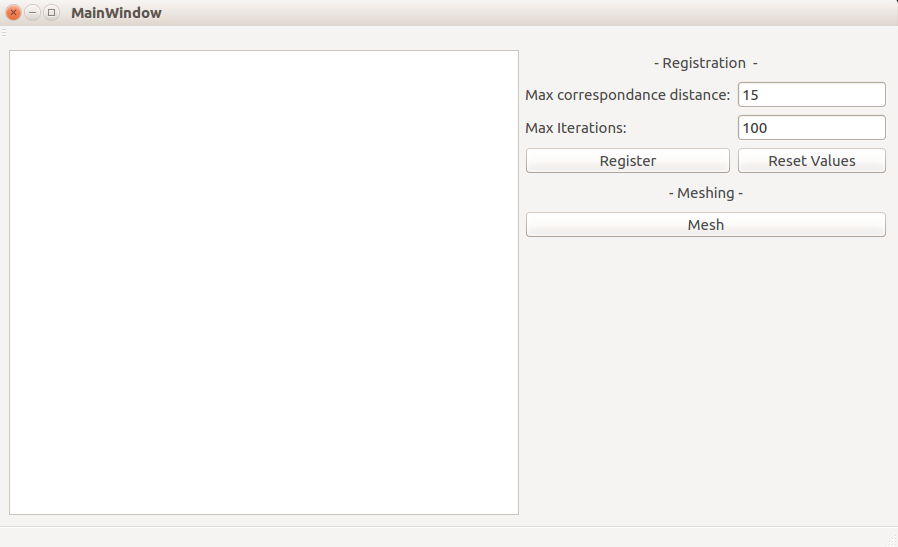
\includegraphics[width=130mm]{figures/3DCopyGUI.PNG}
	\caption{GUI:t för 3DCopy i slutet av iteration 2.}
	\label{fig:3dcopy_gui}
\end{figure}

GUI:t har 5 olika interaktioner som kan utföras. Man kan trycka på någon av de tre knapparna eller skriva i någon av de två input fälten. Det stora vita fältet är till för att visa meddelanden från mjukvaran och kan ej interageras med. Utifrån dessa 5 interaktioner kan vi ta fram EFG:n för GUI:t.

\begin{figure}[H]
	\centering
	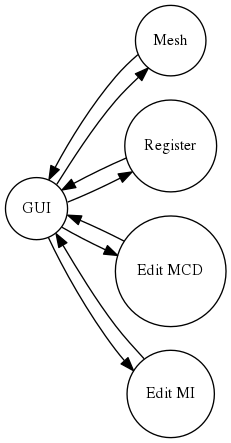
\includegraphics[width=50mm]{figures/3DCopyGUIEFG.png}
	\caption{EFG:n för 3DCopys GUI.}
	\label{fig:3dcopy_guiefg}
\end{figure}

Utifrån EFG:n så ska sedan EIG:n skapas. Det som händer vid skapandet av EIG:n är att noderna GUI, Edit MCD och Edit MI tas bort eftersom att de inte interagerar med systemet.

\begin{figure}[H]
	\centering
	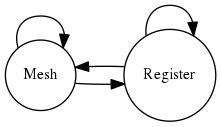
\includegraphics[width=50mm]{figures/3DCopyGUIEIG.png}
	\caption{EIG:n för 3DCopys GUI.}
	\label{fig:3dcopy_guieig}
\end{figure}

Nu när EIG:n är framtagen så ska styrka väljas på testen. För att testerna ska skilja sig lite mer från de testerna utan hänsyn till kontext men åndå inte ta för lång tid så väljs styrka 3 på dessa tester. Det innebär att vi får följande sekvenser som ska användas för att ta fram testfallen.

\begin{table}[h]
	\caption{De sekvenser som ska användas för att ta fram testfallen.}
	\centering
\begin{tabular}{|l|l|}
	\hline
	\textbf{Nr} & \textbf{Sekvens} \\
	\hline
	1 & <Mesh, Mesh, Mesh> \\
	\hline
	2 & <Mesh, Mesh, Register> \\
	\hline
	3 & <Mesh, Register, Mesh> \\
	\hline
	4 & <Mesh, Register, Register> \\
	\hline
	5 & <Register, Mesh, Mesh> \\
	\hline
	6 & <Register, Mesh, Register> \\
	\hline
	7 & <Register, Register, Mesh> \\
	\hline
	8 & <Register, Register, Register> \\
	\hline
\end{tabular}
\end{table}

Dessa sekvenser kombineras sedan för att testfallen ska uppnå 3-cover och 3\textsuperscript{+}-cover och därför också 3\textsuperscript{*}-cover.



\subsection{Testning av 3DCopys GUI utan hänsyn till kontext}

Som test av GUI:t utan hänsyn till kontext kan man tänka sig att en så kallad full-branch coverage kan vara tillräcklig. Det vill säga att alla olika vägar som man kan gå i GUI:t testas. Det blir alltså totalt N! antal test där N är antalet interaktioner som kan utföras på GUI:t.

\section{Resultat}
\label{sec:results-holmberg}

Litteraturstudien visar ett tydligt samband mellan kontexten och vilka fel som testerna lyckas hitta. Kontexten är alltså avgörande för hur interaktionen kommer att påverka mjukvaran.

\section{Diskussion}
\label{sec:discussion-holmberg}

%% Skriv här

\section{Slutsatser}
\label{sec:conclusions-holmberg}

%% Skriv här

%%%%%%%%%%%%%%%%%%%%%%%%%%%%%%%%%%%%%%%%%%%%%%%%%%%%%%%%%%%%%%%%%%%%%%
%%% person-report.tex ends here
